\documentclass[10pt,twocolumn]{article}
\usepackage[margin=0.75in]{geometry}
\usepackage{booktabs,graphicx,hyperref,amsmath}
\usepackage[T1]{fontenc}
\usepackage{lmodern}
\usepackage{xcolor}
\usepackage[section]{placeins}
\hypersetup{colorlinks=true,linkcolor=black,urlcolor=blue!50!black,citecolor=black}
\setlength{\tabcolsep}{4pt}
\newcommand{\CombinedCamera}{2.07}
\newcommand{\CombinedFalse}{0 of 360}
\newcommand{\CombinedSimS}{30.4}
\newcommand{\FtP}{$<$0.001}
\newcommand{\FtSingle}{0.89}
\newcommand{\FtSix}{0.96}
\newcommand{\FtSmallP}{0.481}
\newcommand{\KnockCombinedFalse}{0 of 80}
\newcommand{\KnockProbeFalse}{2 of 80}
\newcommand{\KnockRouterFalse}{2 of 80}
\newcommand{\KnockSensorsFalse}{80 of 80}
\newcommand{\PercLooks}{443}
\newcommand{\PercMean}{4.7}
\newcommand{\PercMedian}{2.4}
\newcommand{\PercWorstMax}{184}
\newcommand{\ProbeCamera}{0.00}
\newcommand{\ProbeSimS}{41.5}
\newcommand{\RouterCamera}{1.19}
\newcommand{\RouterSimS}{30.7}
\newcommand{\SensorsCamera}{0.00}
\newcommand{\SensorsSimS}{22.6}


\title{Vision Can't Feel: Minimal Pairs for Contact-Dependent Robot Success Judgment, and What an Agent Should Check Instead}
\author{Anya Louni}
\date{October 2026}

\begin{document}
\maketitle

\begin{abstract}
Vision-language models (VLMs) are increasingly used to judge whether a robot finished its task. Recent work found these judges near chance when success depends on contact. We study that failure under control. We generate \emph{minimal pairs} in MuJoCo: two snapshots of the same randomized scene, one a success and one a failure that differs by a few millimeters (touching vs.\ hovering, grasped vs.\ beside, seated vs.\ on the rim, pressed vs.\ barely pressed, touching a wall vs.\ short of it). We compare free VLM judges with tiny classifiers on three deliberately degraded, low-cost sensor signals: a fingertip contact switch, gripper effort, and a single-axis wrist force. We also search for the largest physical failure that still fools each VLM. On 400 samples the best free VLM we could run at scale reached 55\% balanced accuracy (95\% CI [50, 60]) with a 54\% false-success rate; a logistic regression on the degraded sensors reached 89\% ([85, 92]) with 11\%. Sensors fail where they cannot observe the contact (push, 50\%) and do not transfer across tasks. Some VLMs still call a failure a success at gaps of several millimeters. Free-tier quotas limited coverage for several models; we report it throughout.

\end{abstract}

\section{Motivation}
A success detector gates retries, rewards, and data collection. A false success is the costly error: the robot moves on while the task silently failed. For contact-dependent tasks the evidence is often a millimeter gap or a force, which a camera at 640 pixels sees poorly or not at all. Cheap sensors measure contact directly. We ask how far that intuition holds when the sensors are realistically noisy, and where it breaks.

\section{Related work}
FailBench~\cite{failbench} evaluates 13 VLM detectors on 2{,}197 real and simulated attempts. Detection is near saturation when success shows as object motion and near chance on contact-rich assembly (no model above 0.60 balanced accuracy on its REASSEMBLE subset), with a bias toward predicting success. It uses vision only and names force-torque as future work. Guardian~\cite{guardian}, AHA~\cite{aha} and RoboFAC~\cite{robofac} train vision-language failure detectors from perturbed demonstrations; all are vision-only. Force and touch appear in policies (e.g.\ force-aware VLAs) rather than as success judges, and classical multimodal anomaly detectors predate VLM judges. To our knowledge no prior work compares cheap non-visual sensors with VLM judges on the same attempts. The vision-side finding is therefore not new; our contribution is the controlled minimal-pair setting, the degraded-sensor comparison, fusion, and the physical attacker. FailBench data was not yet released when we checked, so we could not report on its subset. On the agent side, LLM planners over a fixed skill library with success feedback follow SayCan~\cite{saycan} and Inner Monologue~\cite{innermono}; Inner Monologue already feeds success detection back into the plan. Using touch to decide whether a grasp worked goes back at least to Calandra et al.~\cite{feeling}, and acting to perceive (our press probe) is interactive perception~\cite{interactive}.

\section{Setup}
\paragraph{Simulation.} MuJoCo 3.17 with the Menagerie Franka Panda (gravity compensation, position actuators, damped least-squares IK, guarded moves that stop at 8\,N of tared wrist force). Five tasks, each with a matched failure: \textbf{stack} (held cube touching the base vs.\ hovering), \textbf{grasp} (closed on the cube vs.\ beside it), \textbf{button} (pressed past a 4\,mm click vs.\ less), \textbf{peg} (seated vs.\ on the rim), \textbf{push} (block against a wall vs.\ short of it).
\paragraph{Ground truth.} Explicit rules on simulator state after a 2\,s stability hold with controls frozen: contact force between the right bodies, cap displacement, peg depth plus floor contact, and for grasp a lift test. Images and sensors are captured \emph{before} the hold, at the moment a judge would decide. A pair counts only if its labels come out opposite.
\paragraph{Randomization.} Seeded per pair: key and fill light, table tint, object colors from a palette, three camera poses (one raised oblique, two low profile views), and 0 to 4 distractors kept out of camera sight lines.
\paragraph{Pairs.} Table~\ref{tab:pairs} shows failure magnitudes and the median front-view pixel difference within pairs.
\begin{table}[t]\centering\small\begin{tabular}{lrrr}
\toprule
Task & Pairs & Failure magnitude (mm) & Front pixel diff \\
\midrule
stack & 40 & 0.5--2.0 & 3.6 (median) \\
grasp & 40 & 1.1--3.9 & 24.8 (median) \\
button & 40 & 0.4--2.4 & 5.3 (median) \\
peg & 40 & 0.5--3.9 & 10.3 (median) \\
push & 40 & 0.6--3.0 & 3.7 (median) \\
\bottomrule
\end{tabular}\caption{Scaled set: minimal pairs per task.}\label{tab:pairs}\end{table}
\paragraph{Cheap sensors.} From the simulator at 100\,Hz: fingertip touch (thresholded at 0.3\,N into a binary switch per finger), gripper actuator force (a motor-current proxy), and wrist force along the tool axis only. Degradation per unit strength: switch flips 2\%, 30\,ms latency; effort noise 0.6\,N, 10-bit over $\pm$40\,N, drift up to 0.8\,N; force noise 0.5\,N, 8-bit over $\pm$30\,N, offset up to 1.5\,N, drift up to 1\,N; 2\% dropped samples; 20\,ms latency. Twelve summary features feed logistic regression and a small gradient-boosted tree, trained on 600 samples from seeds disjoint from every test set.
\paragraph{VLM judges.} Free tiers only: Gemini 3.5 Flash, Gemini 3.1 Flash-Lite and Gemma 4 31B through Google AI Studio; Qwen 3.8 27B through Groq; Qwen2.5-VL 3B and Moondream 1.8B through local Ollama on a CPU laptop (images downscaled to 384\,px for these two). Each gets a task description and one front image (single view) or all three views (multi-view), and returns JSON with a verdict and a confidence. Every answer is cached by (model, image hashes, prompt). Calibration uses the stated confidence.
\paragraph{Fusion.} Logistic regression on sensor features plus the VLM's P(success), 5-fold cross-validated on the test set with folds grouped by pair.

\section{Results}
\paragraph{Main comparison.} Table~\ref{tab:large} is the scaled set (400 samples). Table~\ref{tab:small} adds all models and multi-view on the 100-sample set. Free-tier daily quotas stopped some models early; the Coverage column says how many samples each judge answered, and metrics use only those.
\begin{table*}[t]\centering\small\begin{tabular}{lrrrrr}
\toprule
Judge & Coverage & Bal. acc. [95\% CI] & False-succ. [95\% CI] & False-fail. & ECE \\
\midrule
sensor\_gboost & all & 0.89 [0.85, 0.92] & 13\% [8, 17] & 10\% & 0.06 \\
sensor\_logreg & all & 0.89 [0.85, 0.92] & 11\% [7, 16] & 12\% & 0.04 \\
fusion: gemini/gemini-3.1-flash-lite (single) + sensors & 150/400 & 0.88 [0.82, 0.93] & 11\% [4, 19] & 13\% & 0.06 \\
gemini/gemini-3.1-flash-lite (single) & 150/400 & 0.55 [0.51, 0.60] & 53\% [41, 64] & 36\% & 0.45 \\
ollama/moondream:1.8b (single) & 8/400 & 0.50 [0.50, 0.50] & 100\% [100, 100] & 0\% & 0.17 \\
\bottomrule
\end{tabular}\caption{Scaled set (400 samples). Sorted by balanced accuracy.}\label{tab:large}\end{table*}
\begin{table}[t]\centering\small\resizebox{\columnwidth}{!}{\begin{tabular}{lrrrrl}
\toprule
VLM & Shared & Only VLM right & Only sensors right & $p$ & Test \\
\midrule
gemini/gemini-3.1-flash-lite (single) & 164 & 6 & 65 & $<$0.001 & chi2\_cc \\
ollama/moondream:1.8b (single) & 8 & 0 & 3 & 0.250 & exact \\
\bottomrule
\end{tabular}}\caption{Paired McNemar test of each VLM against the sensor classifier on the samples the VLM answered (scaled set).}\label{tab:mcnemar}\end{table}
\begin{table*}[t]\centering\small\begin{tabular}{lrrrrr}
\toprule
Judge & Coverage & Bal. acc. [95\% CI] & False-succ. [95\% CI] & False-fail. & ECE \\
\midrule
fusion: gemini/gemma-4-31b-it (single) + sensors & 83/100 & 0.87 [0.79, 0.94] & 8\% [0, 17] & 19\% & 0.10 \\
sensor\_logreg & all & 0.86 [0.78, 0.93] & 14\% [6, 24] & 14\% & 0.06 \\
sensor\_gboost & all & 0.86 [0.78, 0.93] & 12\% [4, 22] & 16\% & 0.10 \\
fusion: ollama/moondream:1.8b (single) + sensors & 100/100 & 0.86 [0.79, 0.93] & 8\% [2, 16] & 20\% & 0.10 \\
fusion: gemini/gemini-3.1-flash-lite (multi) + sensors & 57/100 & 0.86 [0.76, 0.95] & 10\% [0, 21] & 18\% & 0.12 \\
fusion: gemini/gemini-3.1-flash-lite (single) + sensors & 100/100 & 0.85 [0.77, 0.92] & 8\% [2, 16] & 22\% & 0.13 \\
fusion: ollama/qwen2.5vl:3b (single) + sensors & 100/100 & 0.85 [0.77, 0.92] & 10\% [2, 18] & 20\% & 0.10 \\
fusion: groq/qwen/qwen3.8-27b (single) + sensors & 93/100 & 0.84 [0.75, 0.91] & 11\% [2, 19] & 22\% & 0.11 \\
fusion: gemini/gemini-3.5-flash (single) + sensors & 41/100 & 0.78 [0.65, 0.90] & 24\% [10, 43] & 20\% & 0.18 \\
gemini/gemini-3.1-flash-lite (multi) & 57/100 & 0.65 [0.55, 0.74] & 45\% [28, 62] & 25\% & 0.35 \\
gemini/gemini-3.5-flash (single) & 41/100 & 0.61 [0.48, 0.74] & 52\% [29, 76] & 25\% & 0.34 \\
gemini/gemini-3.1-flash-lite (single) & 100/100 & 0.60 [0.54, 0.66] & 46\% [32, 60] & 34\% & 0.40 \\
groq/qwen/qwen3.8-27b (single) & 93/100 & 0.57 [0.49, 0.65] & 43\% [28, 57] & 43\% & 0.36 \\
gemini/gemma-4-31b-it (single) & 83/100 & 0.56 [0.48, 0.64] & 38\% [23, 53] & 51\% & 0.42 \\
gemini/gemma-4-31b-it (multi) & 9/100 & 0.55 [0.30, 0.80] & 40\% [0, 80] & 50\% & 0.43 \\
ollama/moondream:1.8b (single) & 100/100 & 0.50 [0.50, 0.50] & 100\% [100, 100] & 0\% & 0.23 \\
ollama/qwen2.5vl:3b (single) & 100/100 & 0.50 [0.50, 0.50] & 100\% [100, 100] & 0\% & 0.44 \\
\bottomrule
\end{tabular}\caption{Small set (100 samples), all judges including multi-view. Partial coverage reflects free-tier quotas.}\label{tab:small}\end{table*}
\begin{table}[t]\centering\small\resizebox{\columnwidth}{!}{\begin{tabular}{lrrrrr}
\toprule
Judge & stack & grasp & button & peg & push \\
\midrule
sensor\_gboost & 1.00 & 1.00 & 0.98 & 1.00 & 0.46 \\
sensor\_logreg & 0.94 & 1.00 & 1.00 & 0.99 & 0.50 \\
fusion: gemini/gemini-3.1-flash-lite (single) + sensors & 0.97 & 1.00 & 0.94 & 1.00 & 0.47 \\
gemini/gemini-3.1-flash-lite (single) & 0.47 & 0.68 & 0.59 & 0.59 & 0.41 \\
ollama/moondream:1.8b (single) & -- & 0.50 & 0.50 & 0.50 & 0.50 \\
\bottomrule
\end{tabular}}\caption{Balanced accuracy by task, scaled set.}\label{tab:task}\end{table}
On the scaled set the sensor classifier beats every VLM we ran on balanced accuracy and false-success rate (Table~\ref{tab:large}). The best VLM is gemini/gemini-3.1-flash-lite (single) at 0.55 [0.50, 0.60]; on the 164 samples it answered, a paired McNemar test against the sensor classifier gives $p < 0.001$ (65 samples only the sensors got right, 6 only the VLM got right; Table~\ref{tab:mcnemar}). Fusing it with sensor features gives 0.88 (164/400 samples). On the small set the best VLM is gemini/gemini-3.1-flash-lite (multi) at 0.65 with 57/100 answered; low-coverage rows are indicative only. Vision does best on grasp, where an empty gripper is visible, and worst where the failure is a sub-millimeter gap or a few millimeters of travel.


\paragraph{Where sensors fail.} The single-axis wrist force runs along the tool, so a sideways push barely registers, and the fingertip switch only sees the push if the contact lands inside its zone. Table~\ref{tab:task} shows the push column. Sensor classifiers also do not transfer across tasks (Table~\ref{tab:loto}): a model trained on four tasks is near chance on the fifth, because the same signal means different things in different tasks.
\begin{table}[t]\centering\small\begin{tabular}{lrr}
\toprule
Held-out task & Bal. acc. & False-succ. \\
\midrule
stack & 0.50 [0.50, 0.50] & 100\% [100, 100] \\
grasp & 1.00 [1.00, 1.00] & 0\% [0, 0] \\
button & 0.66 [0.59, 0.74] & 68\% [53, 83] \\
peg & 0.50 [0.50, 0.50] & 100\% [100, 100] \\
push & 0.50 [0.50, 0.50] & 0\% [0, 0] \\
\bottomrule
\end{tabular}\caption{Sensor classifier trained on four tasks, tested on the held-out one.}\label{tab:loto}\end{table}

\paragraph{Noise robustness.} Table~\ref{tab:sweep} and Figure~\ref{fig:sweep} scale every degradation together. Accuracy falls from 0.97 with ideal sensors to 0.89 at the default and 0.50 at strength 32. Its 95\% interval first overlaps the best VLM's at strength 16, and its point estimate falls below the VLM's at strength 32.

\begin{table}[t]\centering\small\begin{tabular}{lrr}
\toprule
Noise strength & Bal. acc. & False-succ. \\
\midrule
0 & 0.97 [0.96, 0.99] & 3\% [1, 5] \\
0.5 & 0.90 [0.87, 0.93] & 10\% [6, 14] \\
1 & 0.89 [0.85, 0.92] & 11\% [7, 16] \\
2 & 0.82 [0.78, 0.86] & 18\% [13, 24] \\
4 & 0.74 [0.70, 0.78] & 20\% [14, 25] \\
8 & 0.66 [0.61, 0.71] & 32\% [25, 38] \\
16 & 0.61 [0.56, 0.65] & 41\% [34, 48] \\
32 & 0.50 [0.45, 0.54] & 54\% [47, 61] \\
\bottomrule
\end{tabular}\caption{Sensor classifier vs.\ noise strength (1 = default cheap hardware).}\label{tab:sweep}\end{table}
\begin{figure}[t]\centering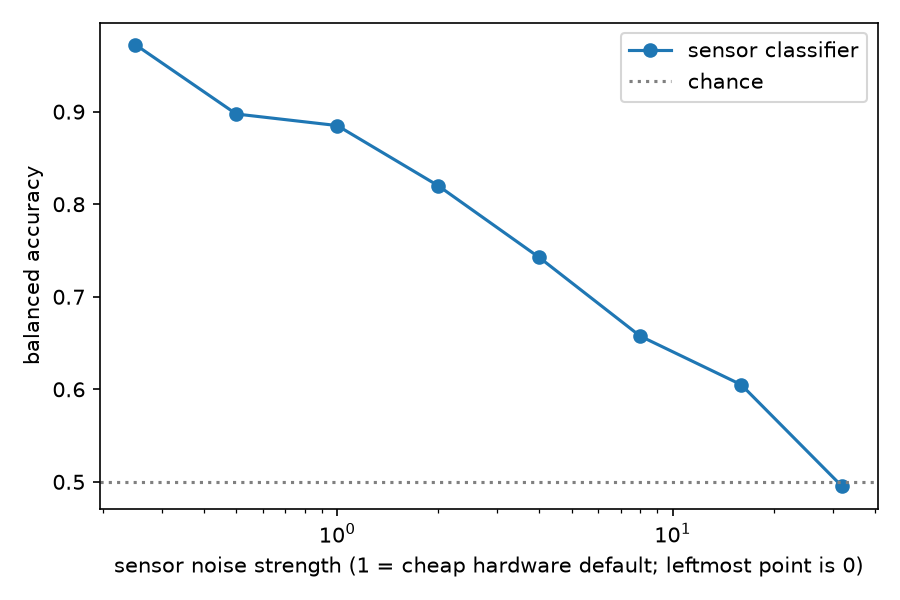
\includegraphics[width=\columnwidth]{../results/large/noise_sweep.png}\caption{Sensor classifier balanced accuracy vs.\ noise strength; dashed: best VLM on the same set.}\label{fig:sweep}\end{figure}

\paragraph{Calibration.} Figure~\ref{fig:rel} plots reliability. VLMs report high confidence whether right or wrong, so their ECE is large (gemini/gemini-3.1-flash-lite (single): 0.45); the sensor classifier's ECE is 0.04.

\begin{figure}[t]\centering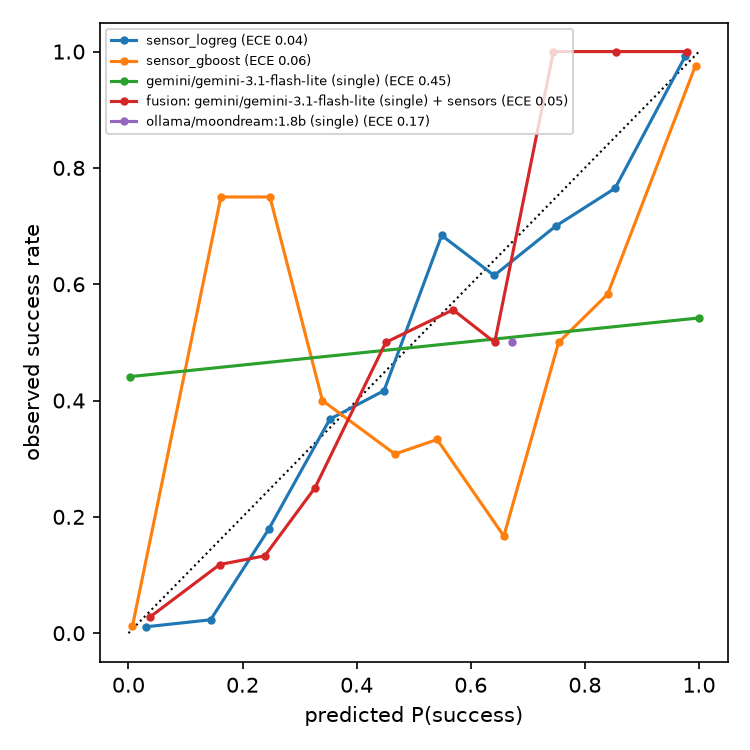
\includegraphics[width=\columnwidth]{../results/large/reliability.png}\caption{Reliability diagrams on the scaled set. VLM confidence is self-reported.}\label{fig:rel}\end{figure}

\paragraph{Millimeters to fool.} For each model, task and scene the attacker climbs a ladder of failure magnitudes (0.5 to 16\,mm; 0.25 to 3.7\,mm below the click for the button), bisects between the largest fooled and smallest not-fooled value, then runs four LLM-proposed mutations (magnitude, light, camera height) that see all previous results. Every candidate is re-simulated and discarded if ground truth turns into success. Table~\ref{tab:attack} reports the largest failure still judged a success, averaged over two scenes; Table~\ref{tab:transfer} re-judges every fooling scene with the other model and the sensor classifier. gemini/gemini-3.1-flash-lite: fooled in 2 of 4 scenes, up to 13.5\,mm. ollama/moondream:1.8b: fooled in 10 of 10 scenes, up to 16.0\,mm. The sensor classifier called 6 of 115 fooling scenes a success.

\begin{table}[t]\centering\small\resizebox{\columnwidth}{!}{\begin{tabular}{lrrrrr}
\toprule
Model & stack & grasp & button & peg & push \\
\midrule
gemini/gemini-3.1-flash-lite & 11.2 & 0.0 & -- & -- & -- \\
ollama/moondream:1.8b & 16.0 & 16.0 & 3.7 & 16.0 & 16.0 \\
\bottomrule
\end{tabular}}\caption{Millimeters to fool (largest failure judged success; mean of 2 scenes).}\label{tab:attack}\end{table}
\begin{table}[t]\centering\small\IfFileExists{tables/transfer.tex}{\begin{tabular}{lr}
\toprule
Judge & Also says success \\
\midrule
gemini/gemini-3.1-flash-lite & 9/41 \\
ollama/moondream:1.8b & 15/15 \\
sensor classifier & 6/115 \\
\bottomrule
\end{tabular}}{Transfer run pending.}\caption{Fooling scenes re-judged by other judges.}\label{tab:transfer}\end{table}

\section{From judging to acting}
The study above judges single snapshots. A robot agent decides many times per task and can act to find out. We
built one: an LLM plans over five skills (move, grasp, lift, place, release) in the style of SayCan and Inner
Monologue~\cite{saycan,innermono}; MuJoCo WASM runs the Panda in a browser; damped least-squares IK executes. The
same cheap sensors check each skill as it runs: a grasp must close both fingertip switches with effort above 5\,N,
a slip turns the switches off, and a placement lowers under a force guard until the wrist force rises. All
experiments in this section use 80 seeded tasks (stack, tower, sort, zone), a scripted planner (no API calls, so
runs are free and repeatable), up to three replans, and true simulator state for scoring. Failures are injected in
the first attempt: a slip while carrying, the target moved just before placing, the cube knocked away right after
release, or seeded random chaos.

\paragraph{Who decides ``done''.} Table~\ref{tab:trials} compares decision rules. An OpenCV detector that fits each
cube's 3D pose from color silhouettes stands in for the camera (the robot then runs open loop, without touch).
Sensors catch failures during the task but are blind after release: alone they declared \KnockSensorsFalse{}
knocked-off episodes a success. Camera and sensors together had \CombinedFalse{} false successes.
\begin{table}[!htb]\centering\small\resizebox{\columnwidth}{!}{\begin{tabular}{lrrrr}
\toprule
Failure & Camera & Sensors & Both & Simulator \\
\midrule
None & 98 [91, 99] & 99 [93, 100] & 99 [93, 100] & 100 [95, 100] \\
Slip & 76 [66, 84] & 99 [93, 100] & 99 [93, 100] & 99 [93, 100] \\
Target moved & 50 [35, 65] & 98 [87, 100] & 98 [87, 100] & 100 [91, 100] \\
Knocked off & 75 [65, 83] & 0 [0, 5] & 79 [69, 86] & 79 [69, 86] \\
Chaos & 93 [85, 97] & 95 [88, 98] & 94 [86, 97] & 96 [90, 99] \\
\bottomrule
\end{tabular}
}\caption{True success (\%, 95\% Wilson interval) by decision rule and failure; 80 episodes per cell, 40 for target moved.}\label{tab:trials}\end{table}

\paragraph{Planning from what the camera sees.} By default the skills aim at true cube poses. In perceived-state
mode they aim at the detector's estimates, refreshed before every attempt. Over \PercLooks{} looks the median
position error was \PercMedian\,mm (mean \PercMean\,mm, worst cube \PercWorstMax\,mm). Table~\ref{tab:perceived}
shows that no rule's true success changed significantly: grasps close on the cube and placements stop on
contact, which absorbs millimeter errors.
\begin{table}[!htb]\centering\small\resizebox{\columnwidth}{!}{\begin{tabular}{lrrrr}
\toprule
Decider, failure & n & Perceived & True state & McNemar \\
\midrule
Simulator, none & 80 & 100 [95, 100] & 100 [95, 100] & 0/0, 1.000 \\
Sensors, none & 80 & 99 [93, 100] & 99 [93, 100] & 1/1, 1.000 \\
Both, none & 80 & 93 [85, 97] & 99 [93, 100] & 0/5, 0.063 \\
Both, chaos & 80 & 90 [81, 95] & 94 [86, 97] & 0/3, 0.250 \\
\bottomrule
\end{tabular}
}\caption{True success (\%) with perceived and true state on the same tasks; McNemar counts only-perceived/only-true correct, and $p$.}\label{tab:perceived}\end{table}

\paragraph{Touch the result before saying done.} Sensors go blind at release, so we added an active check in the
spirit of interactive perception~\cite{interactive}: a \emph{press probe} lowers the closed gripper onto each top
cube and checks, from the noisy wrist force and the arm's own height, that the top face sits where the goal puts
it. A router runs checks cheapest first: sensors; the camera only if the sensors pass; the probe only if the camera
disagrees. Table~\ref{tab:probes} pools all five failure types. Our first probe checked the height where the robot
had put each cube and missed towers rebuilt on a knocked-off middle cube; the current one uses the height the goal
implies (both runs are in the repository). On knocked-off cubes false success fell from \KnockSensorsFalse{} with
sensors alone to \KnockProbeFalse{} with the probe; the remaining misses were towers of the right height in the wrong order, which a press cannot
see and a camera can. The router matched sensors with the probe on true and false success and used \RouterCamera{} camera checks per episode
against \CombinedCamera{} for camera and sensors together, at \RouterSimS{} against \CombinedSimS{} simulated
seconds per episode.
\begin{table*}[t]\centering\small\begin{tabular}{lrrrrrr}
\toprule
Strategy & True success & False success & False, knocked & Sim s & Camera & Probes \\
\midrule
Sensors & 76 [71, 80] & 23 [19, 28] & 100 [95, 100] & 22.6 & 0.00 & 0.00 \\
Sensors + probe & 95 [92, 97] & 1 [0, 2] & 3 [1, 9] & 41.5 & 0.00 & 1.92 \\
Camera + sensors & 93 [90, 95] & 0 [0, 1] & 0 [0, 5] & 30.4 & 2.07 & 0.00 \\
Router & 95 [92, 97] & 1 [0, 2] & 3 [1, 9] & 30.7 & 1.19 & 0.45 \\
\bottomrule
\end{tabular}
\caption{Checking strategies over all five failure types (360 episodes each): true and false success (\%, Wilson interval), false success when the cube was knocked off after release, simulated seconds, camera checks and probes per episode.}\label{tab:probes}\end{table*}

\paragraph{A 6-axis wrist sensor.} We replayed every committed attempt with a 6-axis force/torque sensor at the
wrist (the replayed single-axis traces matched the originals exactly) and gave it the same noise model per axis.
Task-agnostic features (contact onset, peak change, direction relative to the approach, steadiness after onset,
torque) replace the single-axis wrist features; switches and effort stay. On the scaled set balanced accuracy rose
from \FtSingle{} to \FtSix{} (McNemar $p$ \FtP; Table~\ref{tab:ft}), and held-out-task accuracy rose on stack and peg
but not on button or push. On the 100-sample set the logistic-regression gain was not significant ($p$ = \FtSmallP).
With more noise than the default, the advantage disappears: the intervals overlap from twice the default on.
\begin{table}[!htb]\centering\small\resizebox{\columnwidth}{!}{\begin{tabular}{lrrr}
\toprule
Classifier & Single axis & 6-axis F/T & McNemar \\
\midrule
log. reg. & 0.89 [0.85, 0.92] & 0.96 [0.94, 0.98] & 41/12 \\
boosted trees & 0.89 [0.85, 0.92] & 0.96 [0.94, 0.98] & 36/6 \\
held out: stack & 0.50 & 0.89 &  \\
held out: grasp & 1.00 & 1.00 &  \\
held out: button & 0.66 & 0.54 &  \\
held out: peg & 0.50 & 0.86 &  \\
held out: push & 0.50 & 0.50 &  \\
\bottomrule
\end{tabular}
}\caption{Single-axis vs.\ 6-axis wrist sensing, scaled set. McNemar: samples only 6-axis / only single-axis got right.}\label{tab:ft}\end{table}

\paragraph{Can a language model read a touch trace?} Each small-set trace, with the evaluation's noise and printed
at 10\,Hz, went to a text-only model (Table~\ref{tab:trace}). One-shot adds one labelled success/failure pair of the
same task from the training seeds. Zero-shot, the model is worse than the sensor classifier; given one example
pair it is not significantly different from the classifier and clearly better than the camera VLM on the same
samples. Reading a touch trace, given a reference, is within reach of a free text model; reading the gap from an
image is not.
\begin{table}[!htb]\centering\small\resizebox{\columnwidth}{!}{\begin{tabular}{lrrrr}
\toprule
Reader & n & Balanced acc. & False succ. & vs sensor clf. \\
\midrule
gpt-oss-120b (0-shot) & 100 & 0.68 [0.58, 0.78] & 0.18 & 9/27, 0.005 \\
gpt-oss-120b (1-shot) & 96 & 0.91 [0.83, 0.97] & 0.10 & 6/2, 0.289 \\
\bottomrule
\end{tabular}
}\caption{A text LLM judging from the sensor trace alone (small set). Last column: McNemar against the sensor classifier.}\label{tab:trace}\end{table}

\paragraph{Harder instructions.} Twenty hand-written tasks test the planner on relational references, cubes that
start stacked, impossible requests (where the plan schema allows a structured refusal) and distractor phrasing
(Table~\ref{tab:hard}). The LLM planner refused every impossible task and no possible one; the suite proved easier
than intended and does not rank planners.
\begin{table}[!htb]\centering\small\resizebox{\columnwidth}{!}{\begin{tabular}{lrrrrr}
\toprule
Condition & Relational & Reorder & Impossible & Distractor & Correct \\
\midrule
scripted & 5/5 & 4/5 & 5/5 & 5/5 & 95 [76, 99] \\
scripted-chaos & 5/5 & 4/5 & 5/5 & 5/5 & 95 [76, 99] \\
llm & 5/5 & 4/5 & 5/5 & 5/5 & 95 [76, 99] \\
llm-chaos & 4/5 & 4/5 & 5/5 & 5/5 & 90 [70, 97] \\
\bottomrule
\end{tabular}
}\caption{Harder suite: correct per family (goal met, or refusal for impossible tasks). Scripted rows plan from the hand-written goal.}\label{tab:hard}\end{table}

\section{Limitations}
Simulation only; nothing here is validated on hardware, and simulated touch and force are cleaner than real ones even after degradation. The failures are synthetic and drawn from five tasks we designed, so the sensor features fit those tasks; leave-one-task-out results show they do not generalize. The minimal pairs are hard by construction, so VLM accuracy here says little about natural failure distributions. Free-tier quotas limited coverage for several models, and local models ran on downscaled images. VLM confidence is self-reported text, not a probability. We used one prompt per task and did not tune prompts per model. Two scenes per task in the attacker is small. Fusion is cross-validated on the test set rather than trained on separate VLM-labelled data. In the agent experiments the planner is scripted, failures are injected by teleporting cubes or opening the gripper, the probe thresholds were set once and not tuned, and perceived-state mode still gives the planner a scene description from the simulator.

\section{Reproducibility}
Code (MIT), the dataset with images, sensor traces, simulator states, ground truth and every model answer (CC BY 4.0), and a one-command script are public. Cached answers make reruns free.

\begin{thebibliography}{9}\small
\bibitem{failbench} Z.~Navasardyan, T.~Danielyan, H.~Davtyan. FailBench: How Reliable are VLMs at Judging Robot Task Success? arXiv:2609.03611, 2026.
\bibitem{guardian} P.~Pacaud, R.~Garcia, S.~Chen, C.~Schmid. Guardian: Detecting Robotic Planning and Execution Errors with Vision-Language Models. arXiv:2512.01946, 2025.
\bibitem{aha} J.~Duan, W.~Pumacay, N.~Kumar et al. AHA: A Vision-Language-Model for Detecting and Reasoning Over Failures in Robotic Manipulation. arXiv:2410.00371, 2024.
\bibitem{robofac} Z.~Ye, W.~Lu, M.~Ye et al. RoboFAC: A Comprehensive Framework for Robotic Failure Analysis and Correction. arXiv:2505.12224, 2025.
\bibitem{saycan} M.~Ahn, A.~Brohan, N.~Brown et al. Do As I Can, Not As I Say: Grounding Language in Robotic Affordances. arXiv:2204.01691, 2022.
\bibitem{innermono} W.~Huang, F.~Xia, T.~Xiao et al. Inner Monologue: Embodied Reasoning through Planning with Language Models. arXiv:2207.05608, 2022.
\bibitem{interactive} J.~Bohg, K.~Hausman, B.~Sankaran, O.~Brock, D.~Kragic, S.~Schaal, G.~Sukhatme. Interactive Perception: Leveraging Action in Perception and Perception in Action. IEEE Transactions on Robotics 33, 2017.
\bibitem{feeling} R.~Calandra, A.~Owens, D.~Jayaraman et al. More Than a Feeling: Learning to Grasp and Regrasp using Vision and Touch. IEEE Robotics and Automation Letters, 2018.
\end{thebibliography}
\end{document}
